\documentclass[a4paper,10pt]{article}
\usepackage[utf8]{inputenc}

% ----  Useful packages % ---- 
\usepackage{amsmath}
\usepackage{graphicx}
\graphicspath{{images/}}
\usepackage{amsfonts}
\usepackage{amsthm}
\usepackage{amssymb}
\usepackage{makecell}
\usepackage{mathtools}

% ----  Useful packages % ---- 

\usepackage{wrapfig}
\usepackage{caption}
\usepackage{subcaption}
\usepackage{hyperref}
\hypersetup{
	colorlinks,
	citecolor=black,
	filecolor=black,
	linkcolor=black,
	urlcolor=black
}

% ---- Set page size and margins replace ------
\usepackage[letterpaper,top=2cm,bottom=2cm,left=3cm,right=3cm,marginparwidth=1.75cm]{geometry}
% ---- Set page size and margins replace ------

% ------- NOTA ------
\theoremstyle{remark}
\newtheorem{note}{Note}[subsection]
% ------- NOTA ------

% ------- OSSERVAZIONE ------
\theoremstyle{definition}
\newtheorem{observation}{Osservazione}[subsection]
% ------- OSSERVAZIONE ------

% ------- DEFINIZIONE ------
\theoremstyle{plain}
\newtheorem{definition}{Definizione}[subsection]
% ------- DEFINIZIONE ------

% ------- ESEMPIO ------
\theoremstyle{definition}
\newtheorem{example}{Esempio}[subsection]
% ------- ESEMPIO ------

% ------- DIMOSTRAZIONE ------
\theoremstyle{definition}
\newtheorem{demostration}{Dimotrazione}[subsection]
% ------- DIMOSTRAZIONE ------

% ------- TEOREMA ------
\theoremstyle{definition}
\newtheorem{theorem}{Teorema}[subsection]
% ------- TEOREMA ------

% ------- COROLLARIO ------
\theoremstyle{plain}
\newtheorem{corollaries}{Corollario}[theorem]
% ------- COROLLARIO ------

% ------- PROPOSIZIONE ------
\theoremstyle{plain}
\newtheorem{proposition}{Proposizione}[subsection]
% ------- PROPOSIZIONE ------

% ---- Footer and header ---- 
\usepackage{fancyhdr}
\pagestyle{fancy}
\fancyhf{}
\fancyhead[LE,RO]{A.A 2023-2024}
\fancyhead[RE,LO]{Green Computing}
\fancyfoot[RE,LO]{\rightmark}
\fancyfoot[LE,RO]{\thepage}

\renewcommand{\headrulewidth}{.5pt}
\renewcommand{\footrulewidth}{.5pt}
% ---- Footer and header ---- 

% ----  Language setting ---- 
\usepackage[italian, english]{babel}
% ----  Language setting ---- 

\usepackage{listings}
\usepackage{color}

\definecolor{dkgreen}{rgb}{0,0.6,0}
\definecolor{gray}{rgb}{0.5,0.5,0.5}
\definecolor{mauve}{rgb}{0.58,0,0.82}

\lstset{frame=tb,
	language=C,
	aboveskip=3mm,
	belowskip=3mm,
	showstringspaces=false,
	columns=flexible,
	basicstyle={\small\ttfamily},
	numbers=none,
	numberstyle=\tiny\color{gray},
	keywordstyle=\color{blue},
	commentstyle=\color{dkgreen},
	stringstyle=\color{mauve},
	breaklines=true,
	breakatwhitespace=true,
	tabsize=3
}

\definecolor{lightgray}{rgb}{.9,.9,.9}
\definecolor{darkgray}{rgb}{.4,.4,.4}
\definecolor{purple}{rgb}{0.65, 0.12, 0.82}
\lstdefinelanguage{JavaScript}{
	keywords={break, case, catch, continue, debugger, default, delete, do, else, false, finally, for, function, if, in, instanceof, new, null, return, switch, this, throw, true, try, typeof, var, void, while, with},
	morecomment=[l]{//},
	morecomment=[s]{/*}{*/},
	morestring=[b]',
	morestring=[b]",
	ndkeywords={class, export, boolean, throw, implements, import, this},
	keywordstyle=\color{blue}\bfseries,
	ndkeywordstyle=\color{darkgray}\bfseries,
	identifierstyle=\color{black},
	commentstyle=\color{purple}\ttfamily,
	stringstyle=\color{red}\ttfamily,
	sensitive=true
}

\lstset{
	language=JavaScript,
	extendedchars=true,
	basicstyle=\footnotesize\ttfamily,
	showstringspaces=false,
	showspaces=false,
	tabsize=2,
	breaklines=true,
	showtabs=false,
	captionpos=b
}

\title{\textbf{Ingegneria del software}}
\author{Realizzato da: Ghirardini Filippo}
\date{A.A. 2024-2025}

\begin{document}
	\begin{titlepage} %crea l'enviroment
	\begin{figure}[t] %inserisce le figure
		\centering
\includegraphics[width=0.98\textwidth]{marchio_unipi_pant541.png}
	\end{figure}
	\vspace{20mm}
	
	\begin{Large}
		\begin{center}
			\textbf{Dipartimento di Informatica\\ Corso di Laurea Triennale in Informatica\\}
			\vspace{20mm}
			{\LARGE{Corso a Libera Scelta - 6 CFU}}\\
			\vspace{10mm}
			{\huge{\bf Computer Graphics}}\\
		\end{center}
	\end{Large}
	
	
	\vspace{36mm}
	%minipage divide la pagina in due sezioni settabili
	\begin{minipage}[t]{0.47\textwidth}
		{\large{\bf Professore:}\\ \large{Prof. }}
	\end{minipage}
	\hfill
	\begin{minipage}[t]{0.47\textwidth}\raggedleft
		{\large{\bf Autore:}\\ \large{Filippo Ghirardini}}
	\end{minipage}
	
	\vspace{25mm}
	
	\hrulefill
	
	\vspace{5mm}
	
	\centering{\large{\bf Anno Accademico 2023/2024 }}
	
\end{titlepage}
	
	\tableofcontents
	\newpage
	\maketitle
	\begin{center}
		\vspace{-20pt}
		\rule{11cm}{.1pt} 
	\end{center}
	\section{Punto materiale}
Oggetto caratterizzato da una massa [kg] e da un vettore posizione [m] nello spazio 3D.
Dimensioni trascurabili, forma irrilevante rispetto ai fenomeni di interesse.
Vettore posizione come funzione del tempo t[s].
\begin{example}
    Una molecola di ossigeno se sono interessato all'aereodinamica di una vettua. 
    Un satellite attorno alla terra se ignoro le forze di marea.
\end{example}
\hspace{-15pt}\textbf{Un vettore posizione} è una funzione del tempo $t[s]$.
$$\vec{r(t)} = (x(t), y(t), z(t)) = x(t)\hat{x} + y(t)\hat{z} + z(t)\hat{z}$$
\begin{observation}
    I versori cartesiani sono costanti
\end{observation}

\begin{definition}[Legge oraria]
    Si definisce come legge oraria la funzione $t \mapsto \vec{r}(t)$.
\end{definition}

\begin{definition}[Traiettoria]
    Il luogo geometrico di punti visitati dal punto materiale.
    $$\{\vec{r}(t)\:\: per \: t \in \mathbb{R}\}$$
\end{definition}

\begin{example}
    $\vec{r}(t) = (v_0t, y_0, 0)$ e $v_0 = 3m/s, y_o = 5m$ 
    \begin{figure}[h!]
        \centering
        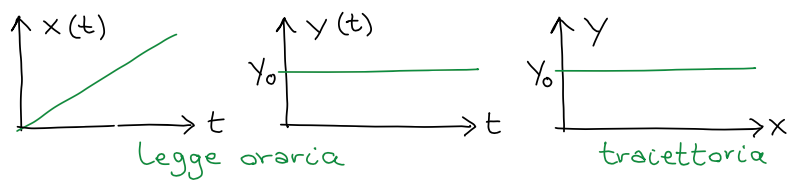
\includegraphics[width=0.8\textwidth]{images/ess-traiettoria.png}
    \end{figure}
\end{example}

\begin{definition}
    La \textbf{velocità istantanea} è la derivata della posizione rispetto al tempo.
    $$v = \lim_{\Delta t \to 0}\frac{\Delta s}{\Delta t} = \frac{ds}{dt}$$
\end{definition}

\begin{definition}
    La \textbf{velocità media} è definita come il rapporto tra lo spostamento e l'intervallo di tempo necessario per effettuarlo.
    $$v_m = \frac{\Delta s}{\Delta t}$$
\end{definition}
\hspace{-15pt}In parole povere è una grandezza che ci dice con quale rapidità cambia la posizione di un punto rispetto al tempo nell'instante $t$.
\subsection*{Vettore velocità}
Derivata rispetto al tempo del vettore posizione e si indica come 
$\frac{d\vec{r}(t)}{dt}\text{ oppure }\dot{\vec{r}}(t)[m/s]$
\begin{equation}
    \begin{split}
    \dot{\vec{r}}(t) & = (\dot{x}(t), \dot{y}(t), \dot{z}(t)) \\
     & = \frac{d}{dt}[x(t)\hat{x} + y(t)\hat{y} + z(t)\hat{z}] \\
     & = \dot{x}(t)\hat{x} + \dot{y}(t)\hat{y} + \dot{z}(t)\hat{z}
    \end{split}
\end{equation}
Per ricavare la forma esplicita uso le proprietà delle derivate (\textbf{linearità}, \textbf{Leibnitz})
\begin{example}
    $\vec{r}(t) = (v_0t, y_0, 0) = v_0t\hat{x} + y_0\hat{y}$ \:\:\:abbiamo che \:\:\:
    $\dot{\vec{r}}(t) = (v_0, 0, 0) = v_0 \hat{x}$
\end{example}
\hspace{-15pt}Velocità e spazio percorso ("integrale di linea").\\
\begin{wrapfigure}[3]{l}{5cm}
    \centering
    \includegraphics[width=5cm]{images/vettore-velocità.png}
\end{wrapfigure}
\begin{align*}
    L & = ||\vec{r}(t_1) - \vec{r}(t_0)|| + ||\vec{r}(t_2) - \vec{r}(t_1)|| + ||\vec{r}(t_3) - \vec{r}(t_2)|| + \dots \\
    & = \sum_i ||\vec{r}(t_{i+1} - \vec{r}(t_i)|| \:\: per\:\: |t_{i+1} - t_i| \text{"piccolo"} \\
    & = \sum_i ||\frac{\vec{r}(t_{i+1}) - \vec{r}(t_i)}{t_{i+1} - t_i}|| (t_{i+1} - t_i) = \int_{t_{in}}^{t_{f_{in}}}||\dot{\vec{r}}(t)||\\
\end{align*}
\begin{example}
    $\vec{r}(t) = (v_0t, y_0)\:\:\: \dot{\vec{r}}(t) = (v_0, 0)$\hspace{15pt}
    $||\dot{\vec{r}}(t)|| = \sqrt{v_0^2 + 0^2} = |v_0|$ \:\:\: $L = |v_0| \cdot (t_{f_{in}} - t_{in})$\\
    Il vettore è costante quindi facendo la derivata torna zero. Con la velocità si calcolo lo spazio percorso ("integrale di linea").
    La differenza fra le posizioni e la differenza dei tempi è il rapporto incrementale in caso gli intervalli siano sufficentemente
    piccoli, da qui si ottiene l'integrale.
\end{example}

\subsection{Vettore accelerazione}
Derivata rispetto al tempo del vettore velocità e si indica con $\frac{d^2\vec{r}(t)}{dt} \text{ oppure } \ddot{\vec{r}}(t) [m/s^2]$
\begin{equation}
    \ddot{\vec{r}}(t) = (\ddot{x}(t), \ddot{y}(t), \ddot{z}(t))\:\: = \:\: \ddot{x}(t)\hat{x} + \ddot{y}(t)\hat{y} + \ddot{z}(t)\hat{z}
\end{equation}
\begin{example}
    $\vec{r}(t)= (\frac{1}{2}a_0t^2, v_0t, 0)$ \hspace{10pt} $\dot{\vec{r}}(t) = (a_0t, v_0, 0)$ \hspace{10pt} $\dot{\vec{r}}(t) = (a_0, 0, 0)$
\end{example}
\hspace{-15pt}Serve perché l'equazione "del moto" di Newton che determinata la legge oraria è formulata in termini di accelerazione.

\subsection{Vettore quantità di moto}
Il prodotto di massa [kg] e velocità [m/s]
$$\vec{p}(t) = m \cdot \dot{\vec{r}}(t) = (m\dot{x}(t), m\dot{y}(t), m\dot{x}(t)) = m\dot{\vec{x}}(t)x + m\dot{\vec{y}}(t)y + m \dot{\vec{z}}(t)z$$
\begin{example}
    Prendiamo un punto di massa 2kg e velocità 3m/s lungo $\hat{x}$.\\
    $p_x(t) = 2 \cdot 3 kg\cdot m/s = 6 kg \cdot m/s$ \hspace{15pt} $p_y(t) = p_z(t) = 0$.
\end{example}
\hspace{-15pt}Serve per generalizzare l'equazione di Newton e per trattare sistemi di piu punti materiali.

\subsection{Vettore momento angolare rispetto a un polo P}
$$\vec{L}_p(t) = m(\vec{r}(t) - \vec{r}_p) \times \dot{\vec{r}}(t)$$
Dove $\vec{r}_p$ è il vettore posizione di p, mentre $\dot{\vec{r}}(t)$ è il prodotto vettoriale.
\begin{example}
    $\vec{r}_p = (l_0, 0, 0)$ \hspace{15pt} $\vec{r}(t) = (v_0t, y_0, 0)$\\
    $\vec{L}_p = m[(v_0t - l_0)\hat{x} + y_0\hat{y}] \times (v_0\hat{x}) \:\: = \:\: m(v_0t - l_0)v_0 \hat{x} \times \hat{x} + my_0v_0\hat{y}\times \hat{x} 
    \:\: = \:\: my_0v_0(-\hat{z}) = (0,0, -my_0v_0)$\\
    Ricorda che $\hat{x} \times \hat{x} = 0$ e $\hat{y} \times \hat{x} = -\hat{z}$
\end{example}
\hspace{-15pt}Il momento angolare dice quanta inerzia ha un oggetto in una rotazione (descrizione sommaria).\\
Il polo P è parte della definizione. È una scelta! Il risultato dipende dal polo.
Serve per formulare l'equazione del moto di sistemi di punti materiali e corpi rigidi.

\subsection{Coordinate polari}
Un metodo per rapprensentare delle cordinate x, y andando a misurare prima la distanza dall'origine e poi si va a vedere
quanto vale l'angolo fra questo segmento dall'asse x, utilizzando seno e coseno.
\begin{wrapfigure}[7]{l}{2cm}
    \centering
    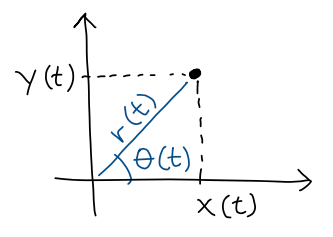
\includegraphics[width=5.5cm]{images/coordinate-polari.png}
\end{wrapfigure}
\begin{align*}
    \begin{cases}
        x(t) = r(t) \cdot \cos(\Theta(t))\\
        y(t) = r(t) \cdot \sin(\Theta(t)) 
    \end{cases}
\end{align*}
\begin{align*}
    \begin{cases}
        r(t) = \sqrt{x(t)^2 + y(t)^2} \geq 0\\
        tg(\Theta(t)) = y(t) / x(t) 
    \end{cases}
\end{align*}
\\
\begin{example} Esempi di rappresentazione di coordinate in coordinate polari.\\
    $x = 0, y = l_0 > 0 \:\: \Rightarrow \:\: r = l_0, \Theta = \pi/2$\\
    $x = 0, y = -l_0 < 0 \:\: \Rightarrow \:\: r = l_0, \Theta = -\pi/2$\\
    $x = l_0, y = l_0 > 0 \:\: \Rightarrow \:\: r = \sqrt{2}l_0, \Theta = \pi/4$\\
\end{example}

\subsection{Versori polari (2D)}
Definisco un versore $\hat{r}(t)$ che punta verso il punto materiale e un versore $\hat{\Theta}(t)$ ortogonale.
Si esprime facilmente in coordinte polari.
$$\vec{r}(t) = (x(t), y(t)) = (r(t)\cos \Theta(t), r(t)\sin\Theta(t)) \:\: = \:\: r(t)(\cos\Theta(t)\hat{x} + \sin\Theta(t)\hat{y})$$
Ma $||\vec{r}(t)|| = |r(t)| = r(t)$ allora definisco $\hat{r}(t) = \vec{r}(t)/ ||\vec{r}(t)|| = \cos \Theta(t)\hat{x} + \sin\Theta(t)\hat{y}$\\\\
Trovo facilmente che un versore ortogonale è:
$$\hat{\Theta(t)} = -\sin\Theta(t)\hat{x} + \cos\Theta(t)\hat{y} \:\:\:\text{infatti} \:\:\: \hat{r}\cdot \hat{\Theta} = c \cdot (-s) + s \cdot c = 0$$
\begin{wrapfigure}[7]{r}{6cm}
    \centering
    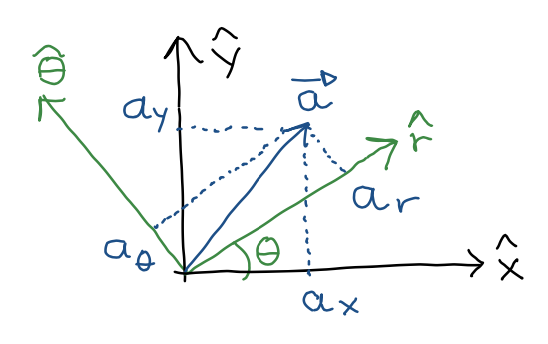
\includegraphics[width=5.5cm]{images/trasformazioni-inverse.png}
\end{wrapfigure}
\begin{note}
    Non c'è legame fra $\Theta$ e $\hat{\Theta}$ è solo una convenzione.
\end{note}
\hspace{-15pt}Le trasformazioni inverse invece si fanno come segue (verifico per sostituzione):
$$\hat{y} = \cos\Theta(t)\hat{r} - \sin\Theta(t)\hat{\Theta} \hspace{20pt} \hat{y} = \sin\Theta(t)\hat{r} + \cos\Theta(t)\hat{\Theta}$$
Possono quindi scrivere ogni vettore nella forma $\vec{a} = a_r\hat{r} + a_{\Theta}\hat{\Theta}$ con le componenti polari $a_r, a_{\Theta}$.
Per evitare ambiguità non scriviamo $(a_r, a_{\Theta})$ e riserviamo la notazione alle componenti cartesiane.\\\\
A differenza dei versori cartesiani quelli polari dipendono dal tempo per costruzioni.
$$\dot{\hat{r}}(t) = \frac{d}{dt}[\cos\Theta(t) \hat{x} + \sin\Theta(t)\hat{y}] \:\: = \:\: -\sin\Theta(t) \cdot \dot{\Theta}(t)\hat{x} + \cos\Theta(t) \cdot \dot{\Theta}(t)\hat{y}$$
Dove $\cos\Theta(t) \cdot \dot{\Theta}(t)$ si applica la derivata della somma, Leibnitz, funzione composta.
$$= \dot{\Theta}(t)\cdot \hat{\Theta}(t) \:\:\:\:(\text{confronto l'espressione di} \hat{\Theta}(t))$$
Similmente $\dot{\hat{\Theta}}(t)= - \dot{\Theta}\hat{r}(t)$.


\subsection*{Vettori posizione, velocità, accelerazione}
$$\vec{r}(t) = r(t)\hat{r}(t)$$
Dove abbiamo che $\vec{r}(t)$ è il vettore, $r(t)$ è una coordinata polare, $\hat{t}(t)$ è il versore polare.
$$\dot{\vec{r}}(r) = \dot{r}(t)\hat{r}(t) + r(t)\dot{\Theta}(t)\hat{\Theta}(t)$$
Dove la parte $\dot{\vec{r}}(r)$ è la velocità radiale.
$$\ddot{\vec{r}}(t) = [\ddot{r}(t) - r(t)\dot{\Theta}(t)^2] \hat{r} + [r(t) \ddot{\Theta}(t) + 2\dot{r}(t)\dot{\Theta}(t)]\hat{\Theta}$$
Nel quale abbiamo che la parte $r(t)\dot{\Theta}(t)^2$ si chiama \textbf{velocità centripeta}, mentre $2\dot{r}(t)\dot{\Theta}(t)$ si dice \textbf{accelerazione di Coriolis}.


	% !TeX spellcheck = it_IT
\newpage
\section{Processo software}
\begin{definition}[Processo software]
	Sequenza di attività necessarie a sviluppare un sistema software.
\end{definition}
\noindent Ogni modello di processo software include:
\begin{itemize}
	\item \textbf{Specifica}: definizione di cosa deve essere fatto
	\item \textbf{Progettazione} e \textbf{implementazione}
	\item \textbf{Validazione}: verifica che il sistema rispetti le specifiche
	\item \textbf{Evoluzione}: modifica o aggiornamento del sistema
\end{itemize}

\subsection{Fasi di sviluppo}
\subsubsection{Specifica}
Questa fase stabilisce quali \textbf{servizi} sono richiesti e quali \textbf{vincoli} ci sono. È quindi un processo di \textit{ingegneria dei requisiti}:
\begin{itemize}
	\item \textbf{Estrazione} e \textbf{analisi} dei requisiti: cosa richiedono o si aspettano gli stakeholder
	\item \textbf{Specifica} dei requisiti: definirli in dettaglio
	\item \textbf{Convalida} dei requisiti: verificare che siano validi
\end{itemize}
\begin{center}
	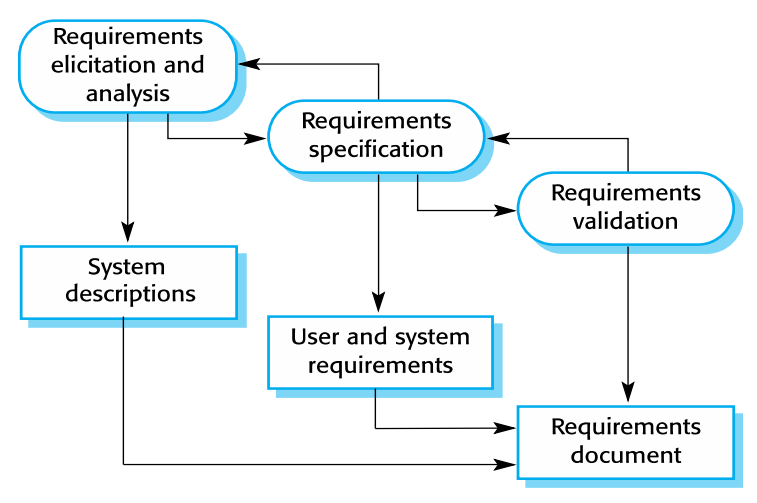
\includegraphics[scale=0.4]{specifica.png}
\end{center}

\subsubsection{Progettazione}
In questa fase si definisce una struttura software che realizzi la specifica, analizzando quattro aspetti:
\begin{itemize}
	\item \textbf{Architectural design}: identificazione della struttura in termini di componenti e di come si relazionano tra di loro
	\item \textbf{Database design}: definizione delle strutture dati necessarie e della loro rappresentazione in database
	\item \textbf{Interface design}: definizione delle interfacce tra le diverse componenti del sistema
	\item \textbf{Component design}: definizione in dettaglio delle varie componenti, identificando quelle realizzabili con elementi già esistenti
\end{itemize}
\begin{center}
	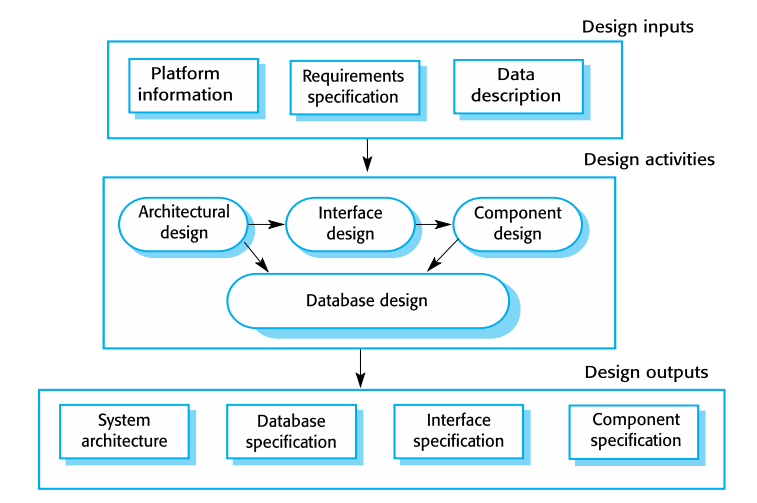
\includegraphics[scale=0.4]{prog.png}
\end{center}

\subsubsection{Sviluppo}
La struttura progettata nella fase precedente viene ora realizzata tramite uno o più applicativi da implementare o da configurare. Include:
\begin{itemize}
	\item \textbf{Programmazione} attività senza un processo standard
	\item \textbf{Debugging}: attività per identificare e correggere errori o bug
\end{itemize}
Spesso la progettazione e lo sviluppo sono svolte in \textbf{interleaving}.

\subsubsection{Validazione}
\textbf{Verifica} e \textbf{validazione} hanno lo scopo di dimostrare che un sistema è conforme alle specifiche e soddisfa i requisiti del cliente. Viene spesso fatta tramite \textbf{testing} con casi derivati dalla specifica dei dati che poi dovranno essere realmente utilizzati. Si suddivide in:
\begin{itemize}
	\item \textbf{Component} testing: i componenti sviluppati sono testati indipendentemente
	\item \textbf{System} testing: il sistema è testato interamente prestando particolare attenzione alle \textit{emergent properties}
	\item \textbf{Customer} testing: il sistema è testato con i dati del cliente
\end{itemize}
\begin{center}
	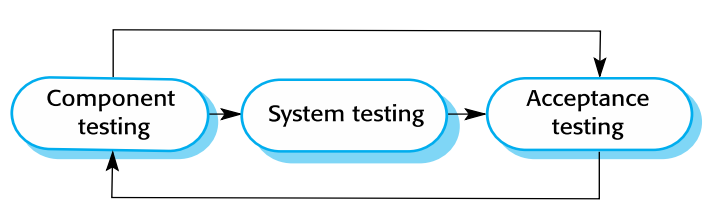
\includegraphics[scale=0.4]{valida.png}
\end{center}

\subsubsection{Evoluzione}
I cambiamenti sono inevitabili in quanto le richieste del cliente possono cambiare nel tempo o possono uscire nuove tecnologie più aggiornate. Questi portano a dei \textbf{rework} costosi che richiedono la ripetizione parziale delle fasi precedentemente descritte.\\
Per ridurre i costi è importante anticipare i cambiamenti e garantire quindi \textbf{change tolerance}. Questo è più facile con i modelli incrementali.

\subsection{Modelli}
\begin{definition}[Modello]
	Il modello di un processo software fornisce una rappresentazione astratta del processo stesso:
	\begin{itemize}
		\item \textbf{Suddivisione} del processo in attività: cosa fare, quando farlo, come e cosa si ottiene
		\item \textbf{Organizzazione} delle attività: ordinamento, criteri di terminazione
	\end{itemize}
	E.g. ISO 12207
\end{definition}

\subsubsection{Sequenziale}
\paragraph{Build and fix}
Questo modello non prevede alcuna specifica o progettazione: lo sviluppatore scrive un programma e lo modifica ripetutamente finché non soddisfa il cliente. Adeguato solo per progetti molto piccoli.
\begin{center}
	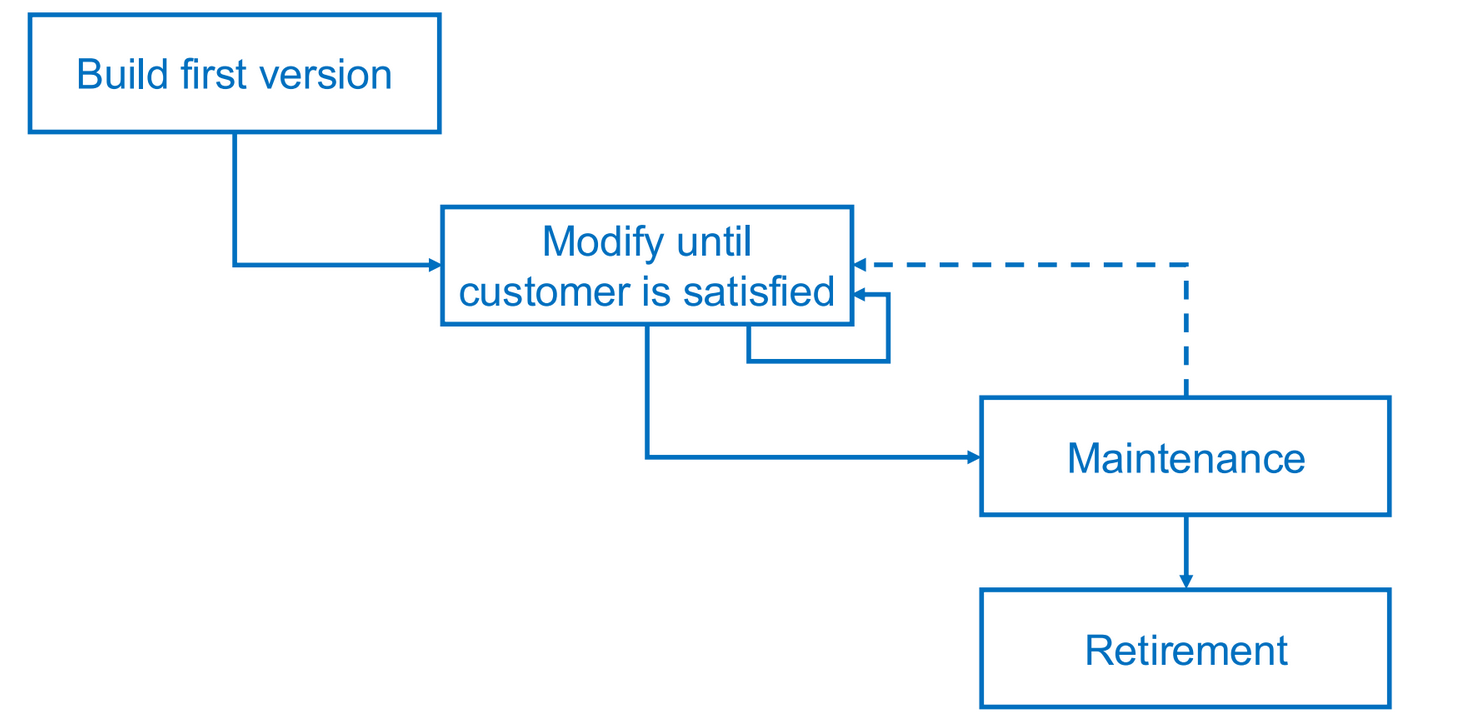
\includegraphics[scale=0.15]{buildfix.png}
\end{center}

\paragraph{Modello a cascata}
Modello ideato da Royce nel 1970, fu il primo a distinguere e definire le fasi di un processo software, dando finalmente importanza all'analisi e alla progettazione prima della codifica.\\
Ogni fase prima di procedere deve produrre un documento che deve essere approvato da chi di dovere.\\
I \textbf{contro} principali sono l'enorme quantità di \textit{documenti} prodotti e l'estrema \textit{rigidità}: il cliente vede solo il prodotto finale che spesso non va bene e si deve rincominciare da capo.

\begin{center}
	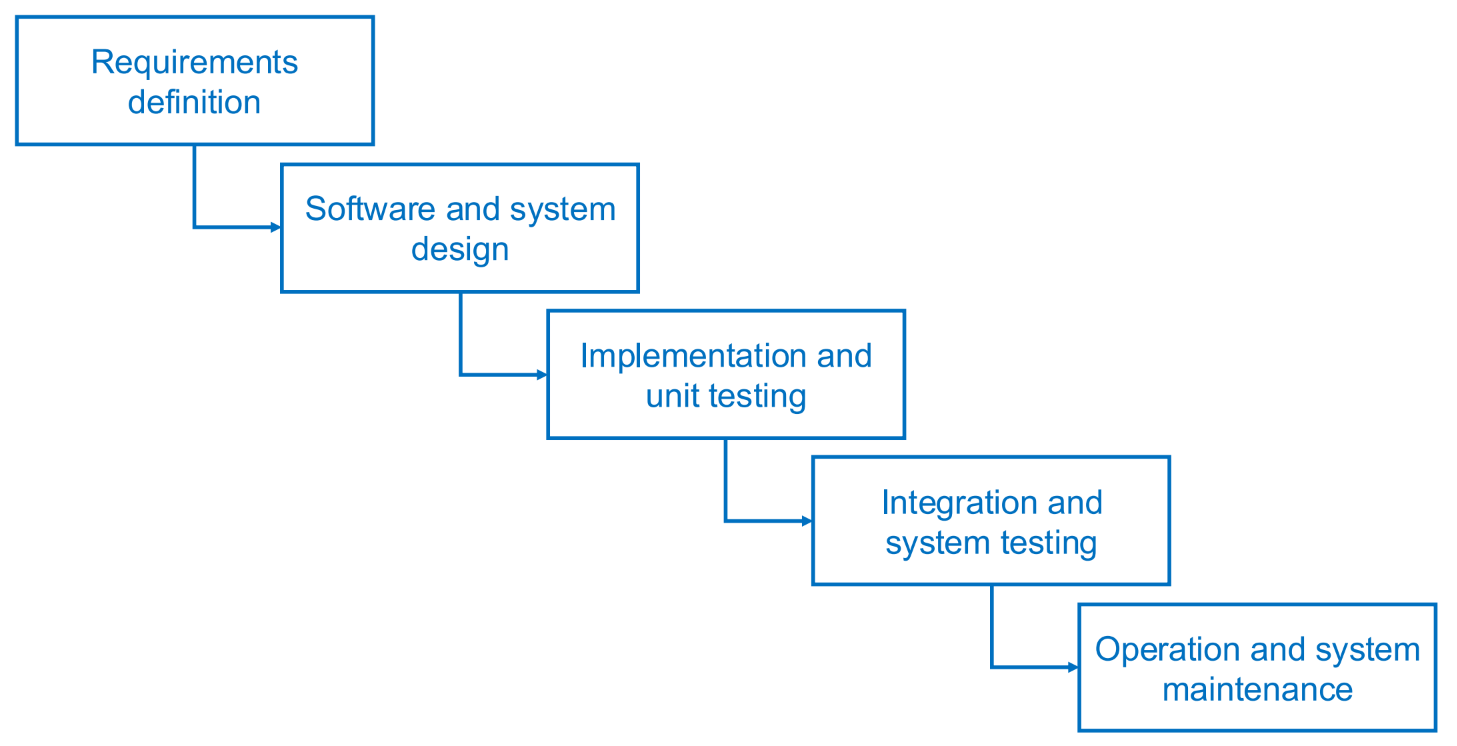
\includegraphics[scale=0.15]{royce.png}
\end{center}

\begin{note}
	Royce stesso riconosce i problemi del suo modello e propone un alternativa con un \textbf{feedback loop} da una fase alla precedente.
\end{note}

\paragraph{Modello a V}
In questo modello le attività di \textbf{sinistra} sono di analisi che scompongono i requisiti degli utenti in sezioni piccole; quelle di \textbf{destra} aggregano e testano il prodotto delle precedenti per verificare che le esigenze siano effettivamente rispettate.\\
Al centro troviamo la progettazione dei \textbf{test} da eseguire prima della codifica.
\begin{center}
	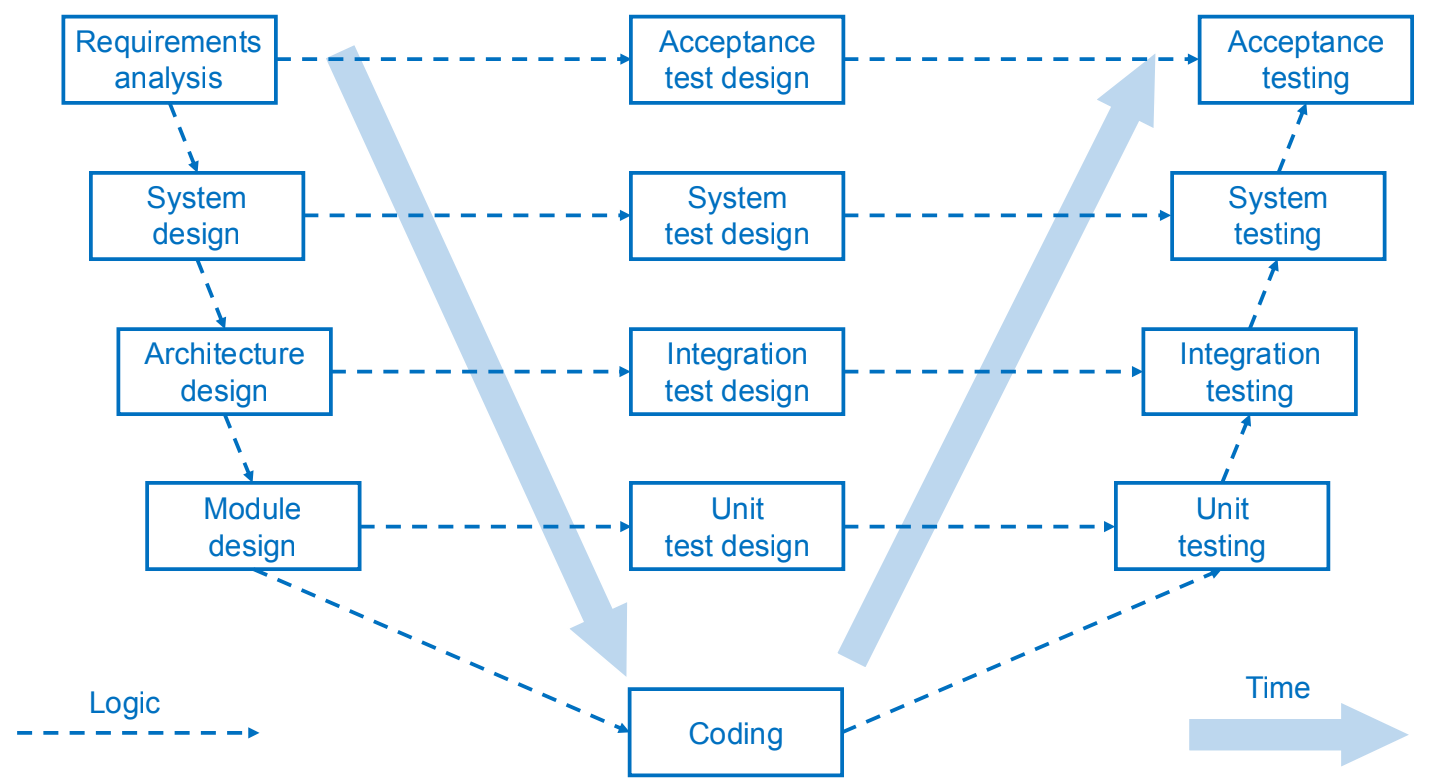
\includegraphics[scale=0.3]{Vmodel.png}
\end{center}

\begin{note}
	Questo modello è uno standard SQA (qualità del software).
\end{note}

\subsubsection{Iterativo}
\paragraph{Rapid prototyping o evolutivo}
Consiste nel costruire velocemente un prototipo per permettere al committente di sperimentarlo. In questo modo il cliente può descrivere meglio i requisiti, sopratutto quando anche a lui non sono chiari.
\begin{center}
	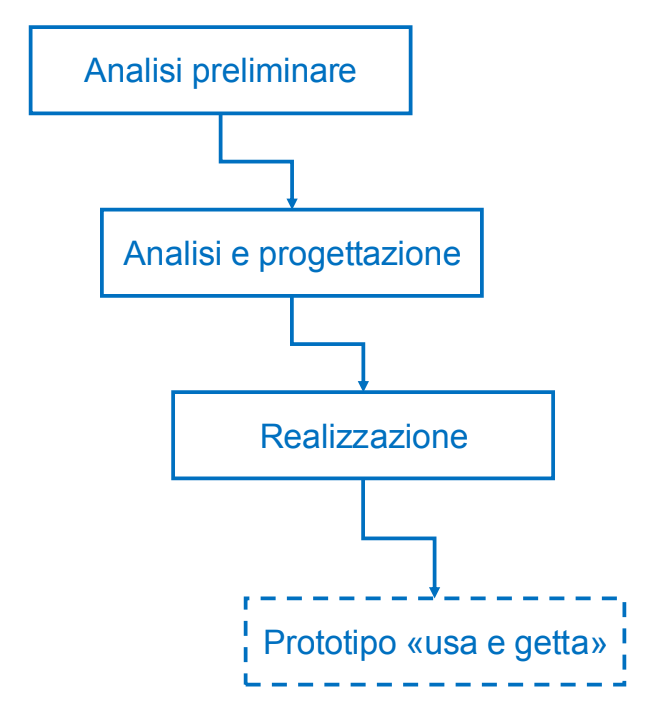
\includegraphics[scale=0.3]{rapidproto.png}
\end{center}

\paragraph{Modello incrementale}
In questo modello il sistema è costruito \textbf{iterativamente} aggiungendo nuove funzionalità a partire da requisiti definiti inizialmente.\\
Questo permette di \textbf{ritardare} fasi che per motivi esterni non possono proseguire e fa uscire versioni iniziali ed utilizzabili molto rapidamente, in modo da ricevere anche \textbf{feedback} che aiutino a correggere il prodotto a basso costo.\\
I contro principali sono che il processo di sviluppo non è molto visibile e c'è il rischio che diventi un \textit{build and fix}: la struttura del sistema tende a degradarsi e diventa più costoso fare il refactoring.

\begin{center}
	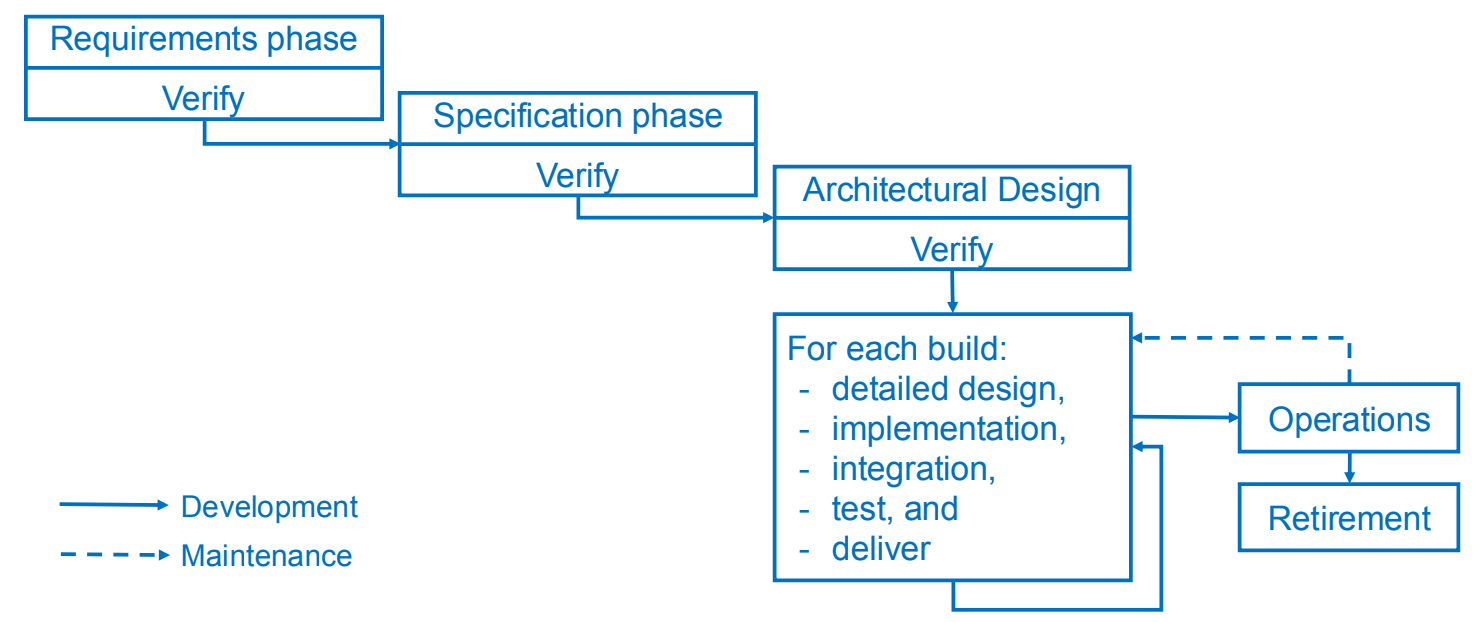
\includegraphics[scale=0.3]{incrementale.png}
\end{center}

\paragraph{Modello a spirale}
Ideato da Bohem nel 1998, ispirato dal \textit{plan-do-check-ackt} di Deming, divide ogni \textbf{iterazione} in quattro fasi:
\begin{enumerate}
	\item Definizione degli obiettivi
	\item Analisi dei rischi
	\item Sviluppo e validazione
	\item Pianificazione del nuovo ciclo
\end{enumerate}
È un modello astratto da istanziare decidendo cosa fare in ogni iterazione e in ogni fase, applicandolo volendo ai cicli tradizionali. Si concentra molto sugli aspetti gestionali: pianificazione delle fasi, \textbf{risk-driven} (guidato dall'analisi dei rischi) e comunicazione con il cliente.

\begin{center}
	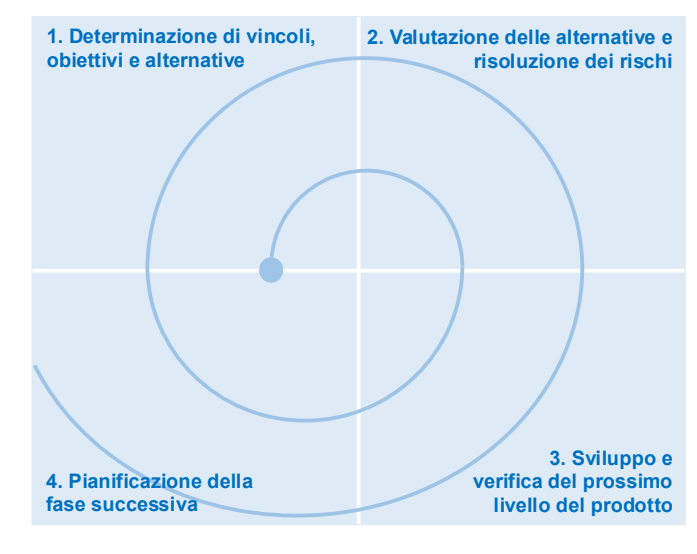
\includegraphics[scale=0.4]{spirale.png}
\end{center}

\paragraph{Unified process}
Ideato da Booch Et Al nel 1999, è guidato da \textbf{casi d'uso} e \textbf{analisi dei rischi} già a partire dalla raccolta e analisi dei requisiti. È un modello iterativo \textbf{incrementale} incentrato sull'\textbf{architettura}: nelle prime fasi c'è una definizione generale e i dettagli vengono lasciati alle fasi successive. Questo permette di avere subito una visione generale del sistema che diventa poi facilmente adattabile.
\begin{center}
	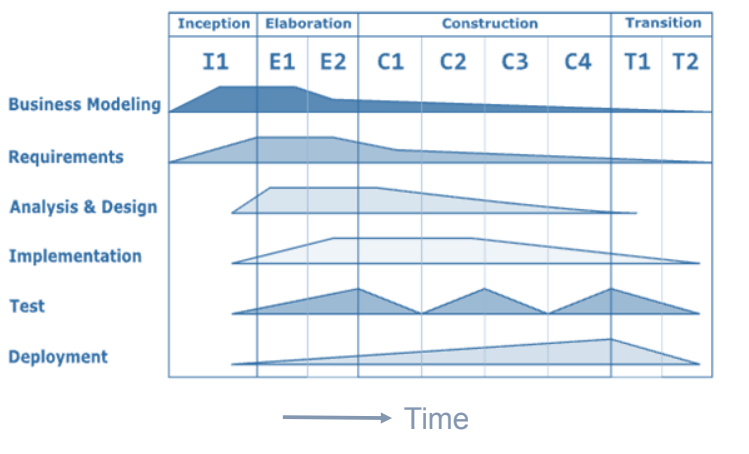
\includegraphics[scale=0.5]{unifproc.png}
\end{center}

\subsubsection{Agile}
Oggi è sempre più importante la \textbf{rapidità} nello sviluppo e nel rilascio del software in quanto i requisiti delle aziende cambiano molto velocemente e con essi diventa impossibile avere un sistema stabile di requisiti.\\
Il modello agile viene introdotto negli anni '90 proprio per ridurre i tempi sopra descritti:
\begin{itemize}
	\item Le fasi di specifica, progettazione e sviluppo sono eseguite in \textbf{interleaving}
	\item Il sistema è sviluppato con versioni incrementali valutate assieme agli stakeholder
	\item Rilascio frequente
	\item Supporti allo sviluppo, e.g. automated testing
\end{itemize}
\begin{center}
	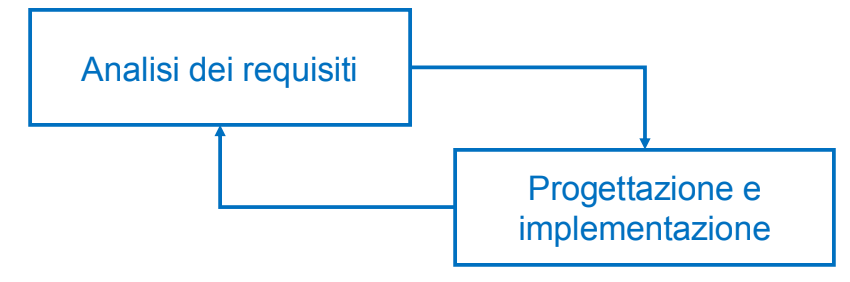
\includegraphics[scale=0.3]{agile.png}
\end{center}

Il modello agile segue i seguenti principi:
\paragraph{Customer involvement} I clienti devono essere coinvolti durante il processo di sviluppo per fornire, prioritizzare e valutare le iterazioni del sistema.
\paragraph{People not process} Le abilità del team devono essere riconosciute e gli sviluppatori devono essere liberi di sviluppare a modo loro, purché venga mantenuta comunicazione.
\paragraph{Mantain semplicity} Cercare di ridurre sempre al minimo la complessità nello sviluppo e nel sistema. Bisogna mantenere il codice semplice ma avanzato tecnicamente a discapito di una documentazione mantenuta al minimo.
\paragraph{Incremental delivery} Il sistema software è sviluppato in versioni incrementali, con il cliente che specifica i requisiti da soddisfare in ciascuna versione.
\paragraph{Embrace change} Accettare che i requisiti cambieranno nel tempo e rendere facile la loro implementazione.\\\\

Il modello agile è \textbf{conveniente} per lo sviluppo di prodotti di piccola o media dimensione (fino a $50$ sviluppatori) oppure in contesti di sviluppo di sistemi custom (meno regolamenti e restrizioni).\\
Nella pratica comunque viene usato nella maggior parte dei team.\\\\

\noindent Il modello agile ha portato alla nascita di:
\begin{itemize}
	\item \textbf{Continuous Integration}: integrazione continua di tutte le modifiche o aggiunte all'interno di un \textit{main branch}, validata tramite automatic build e testing
	\item \textbf{Continuous deployment}: dispiegamento continuo e \textit{automatico} delle nuove versioni ottenute tramite CI
\end{itemize}

\subsubsection{Extreme Programming}
L'extreme programming è un approccio estremo all'approccio iterativo e agile. Prevede che nuove versioni minori siano rilasciate più volte in un giorno, versioni incrementali rilasciate al cliente ogni due settimane e tutti i test sono eseguiti per ogni build.
\begin{center}
	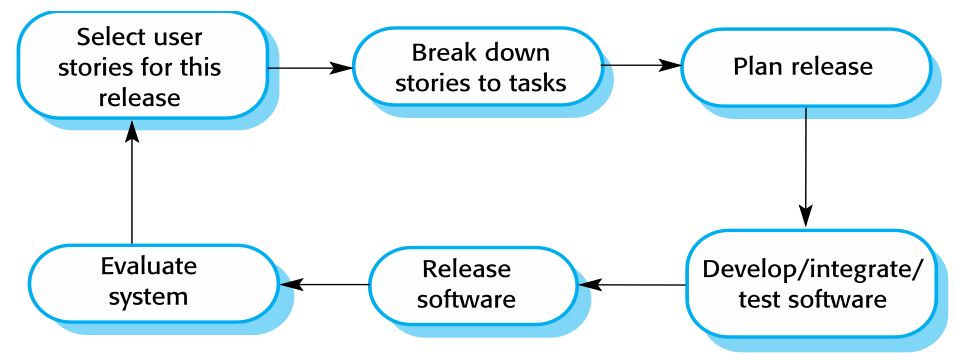
\includegraphics[scale=0.35]{xp.png}
\end{center}

\noindent Alcune pratiche comuni nell'XP:
\paragraph{Planning incrementale} I requisiti sono raccolti sotto forma di user stories divise in \textbf{task}. Quelle da includere nella release sono determinate in base al tempo disponibile e alla loro priorità.
\paragraph{Release piccole} Si parte con una piccola release iniziale che garantisca le funzionalità di base si procede con piccole e frequenti release che aggiungono funzionalità.
\paragraph{Design semplice} La progettazione si concentra solo sui requisiti correnti e deve essere comprensibile a tutti.
\paragraph{Test-first developement} Si sviluppano prima i test del codice stesso (a volte generati automaticamente).
\paragraph{Refactoring} Il refactoring deve essere eseguito continuamente appena ci si rende conto del miglioramento necessario, mantenendo sempre il codice semplice, facilmente manutenibile e auto esplicativo.
\paragraph{Pair programming} Gli sviluppatori lavorano in coppia in modo che ci sia sviluppo e supporto reciproco.
\paragraph{Collective ownership} Le coppie lavorano su tutte le aree del sistema e la responsabilità è quindi condivisa.
\paragraph{Sustainable pace} Ridurre al minimo il lavoro straordinario in quanto abbassa qualità e produttività.
\paragraph{On-site customer} Un rappresentante del cliente deve essere disponibile al team per fornire o prioritizzare i requisiti.\\\\

Il modello di Extreme Programming si concentra principalmente su aspetti tecnici e per questo non è facilmente integrabile nelle organizzazioni. Di conseguenza il metodo non è molto diffuso ma alcuni degli aspetti che tratta sono stati trasportati in altri approcci.

\subsubsection{Scrum}
Scrum è un metodo agile per lo sviluppo iterativo e incrementale di un sistema software. L'idea è di ottenere un processo in cui un insieme di persone si muovono all'unisono per raggiungere un obiettivo che soddisfi la squadra.
\begin{definition}[Product backlog]
	Documento che contiene tutti i requisiti attualmente conosciuti.
\end{definition}
Ci sono tre figure coinvolte:
\begin{itemize}
	\item \textbf{Product owner}: chi identifica le caratteristiche del prodotto, decide le priorità e revisiona il \textbf{product backlog} per assicurarsi che vengano rispettati i requisiti
	\item \textbf{Scrum master}: figura responsabile di assicurare che il processo avvenga efficacemente, garantendo le condizioni ambientali e motivazionali al meglio assicurandosi che non ci siano interferenze esterne (senza però avere autorità sul team)
	\item \textbf{Developement team}: gruppo autogestito di sviluppatori non più grande di 7 persone che si occupa dello sviluppo e della documentazione
\end{itemize}
Le fasi del metodo scrum sono:
\begin{enumerate}
	\item \textbf{Pre-game phase}, ovvero la pianificazione, che a sua volta si compone di:
	\begin{itemize}
		\item \textbf{Planning sub-phase}: definizione del sistema che deve essere sviluppato in termini di product backlog
		\item \textbf{Architecture sub-phase}: design di alto livello del sistema, inclusa l'architettura, in base agli elementi del backlog
	\end{itemize}
	\item \textbf{Game phase}, ovvero lo sviluppo. Il sistema viene sviluppato attraverso una serie di \textbf{sprint}, ovvero un ciclo iterativo nel quale vengono sviluppate o migliorate delle funzionalità. Ogni sprint dura da una settimana ad un mese e include le classiche fasi di sviluppo. Si divide nelle seguenti fasi:
	\begin{enumerate}
		\item Si parte dal product backlog che contiene la lista dei \textbf{requisiti} da fare (TBD). Da questi vengono selezionati dal team e dal cliente quelli da sviluppare.
		\item Si procede con la pianificazione, gestita dal product owner, e con la creazione dello \textbf{sprint backlog}
		\item Inizia lo sviluppo da parte dei diversi team che rimangono isolati e protetti dallo scrum master; si occupa anche di organizzare brevi meeting giornalieri di aggiornamento.
		\item Al termine dello sprint il prodotto viene revisionato in un incontro tra team, clienti ed eventuali utenti
		\item Tra uno sprint ed il successivo viene organizzato un evento di \textbf{retrospettiva} dove il team riflette, impara e si adatta con l'obiettivo di migliorare
	\end{enumerate}
	\item \textbf{Post-game phase}: conclude il processo di sviluppo e il prodotto viene preparato per il rilascio (test, integrazione, documentazione, formazione e marketing)
\end{enumerate}
I vantaggi di questo approccio sono che il prodotto e \textbf{partizionato} in sotto problemi più facili da gestire, i requisiti non ancora pronti non ostacolano lo sviluppo, c'è molta comunicazione, i clienti ottengono increment periodici e si stabilisce un rapporto di fiducia.

\subsection{Kanban}
Il Kanban è un approccio all'organizzazione di un progetto che consiste nel dividere le attività tra \textbf{To Do}, \textbf{Work In Progress} e \textbf{Done}. Questi vengono poi visualizzati tramite una tabella. Viene inoltre imposto un limite alla categoria WIP che riduce il \textbf{task switching} e rende più facile trovare i colli di bottiglia. Ottimizza in generale l'\textbf{efficienza}.
\end{document}
